\section{Evaluation of Topic Quality}
\label{sec:eva}

Accurate identification of tweet topic is important for analysis of topic dynamics because each tweet performs as a unit to form the component of topics a day. If every tweet is assigned with noisy topics, the significance of main topic will decrease while weight of minor topics may increase. Different from conventional LDA, because of the limitation of tweet length, we assign only one topic for each tweet in the \stlda model. Meanwhile we train news and tweets together so that topics of news and tweets are comparable. In this section, we compare topic quality by LDA and \stlda to prove that \stlda gives reasonable good results and performs better than LDA for analysis of topic dynamics. The hyperparameters $\alpha$ and $\beta$ are both set to 0.1 and the number of topics is set to 10. As topics given by the two models are in different orders, we match topics based on KL divergence before comparing them. The matching procedure starts by obtaining a KL divergence table $T$. Each cell $T_{k_1,k_2}$ stores the KL divergence of topic $k_1$ given by LDA and topic $k_2$ given by \stlda as

\begin{eqnarray}
T_{k_1,k_2}&=&\mathrm{KL}(\bm{\phi_{k_1}^\mathrm{LDA}}||\bm{\phi_{k_2}^\mathrm{\stlda}})\\
&=&\sum_{v=1}^{V} \phi_{k_1,v}^{\mathrm{LDA}} \log_2 \frac{\phi_{k_1,v}^{\mathrm{LDA}}}{\phi_{k_2,v}^{\mathrm{\stlda}}}.
\end{eqnarray}

Then we run a depth-first search algorithm on the KL divergence table to find the best match with smallest overall KL divergence. Meanwhile if one pair has KL divergence larger than a threshold, there is no matching topic.

\subsection{Balanced Topics from Tweets and News}

\begin{table*}[htpb]
\centering
\begin{threeparttable}
\begin{tabular}{|c|c|l|}
\hline
\bf \tabincell{c}{Model\\(Corpus)} & \bf Topic & \multicolumn{1}{c|}{\bf Top Words}\\ \hline
\multirow{5}*{\tabincell{c}{LDA\\(NT)\tnote{1}}} & Obama Talk & \tabincell{l}{happen, i'm, make, thing, talk, situation, what's, what's\_happen, bad, you're\\\wycomment{Does this topic really belong to \obamatalk?}}\\ \cline{2-3}
 & Protest & tear\_gas, protester, arrest, fire, medium, rt, protestor, street, crowd\\ \cline{2-3}
 & Racist & black, white, loot, protect, community, racist, stop, race, citizen, riot\\ \cline{2-3}
 & Curfew & missouri, state, obama, national\_guard, call, curfew, mo, press, governor\\ \cline{2-3}
 & Pray & peace, pray, justice, stand, love, tonight, hope, stay, family, safe\\ \hline
\multirow{5}*{\tabincell{c}{\stlda\\(NT)}} & Obama Talk & obama, president, law\_enforcement, house, holder, make, story, post, include\\ \cline{2-3}
 & Protest & tear\_gas, arrest, protester, fire, rt, reporter, medium, shoot, crowd\\ \cline{2-3}
 & Racist & black, white, make, race, america, obama, stop, happen, situation, riot\\ \cline{2-3}
 & Curfew & missouri, curfew, state, national\_guard, governor, nixon, call, gov, order\\ \cline{2-3}
 & Pray & peace, pray, stand, justice, night, love, tonight, today, family\\ \hline
\multirow{5}{*}{\tabincell{c}{LDA\\(N)\tnote{2}}} & Obama Talk & obama, president, house, make, white, news, national, deal, run, defense\\ \cline{2-3}
 & Protest & st\_louis, nixon, protester, shooting, county, justice, aug., investigation, state, thursday\\ \cline{2-3}
 & Racist & black, make, white, cop, time, don't, year, good, man, thing\\ \cline{2-3}
 & Curfew & protester, johnson, tear\_gas, crowd, curfew, night, fire, street, missouri, shoot\\ \cline{2-3}
 & Pray & (No matching topic)\\ \hline
\end{tabular}
\begin{tablenotes}
\footnotesize
\item[1] NT: news and tweets.
\item[2] N: news only.
\end{tablenotes}
\caption{Topic Examples}\label{tab:topic}
\end{threeparttable}
\end{table*}

To make sure that \stlda has balanced topics that come from both tweets and news, we train another model merely on news and set the results as a baseline for comparison. Table~\ref{tab:topic} shows four common topics for all three models and one topic that only exists in results trained on news and tweets together. Four common topics indicate that news topics are kept when mixture of documents are trained together. But there is no matching topic in the baseline results corresponding to the topic \pray in LDA and \stlda on NT, which means \pray tends to only exists in tweets. Meanwhile top words in the four common topics are different. Emergence of Twitter language such as \emph{rt} and \emph{gov} in top words indicate topics from tweets. So \stlda can extract topics from both news and tweets, not biased to one type of texts, and it discovers topics that exist in both news and tweets.

\subsection{Topic Quality for Tweets}
\label{subsec:intrinsic}
Accurate topic assignment is important for analysis of topic dynamics. In this part we pick several tweets and evaluate quality of topic assignment by \stlda. We list five tweets in Table~\ref{tab:tweets} and manually labeled with the main topic. Topic assignments by LDA and \stlda are given in Table~\ref{tab:tweet_topic}. Topics in LDA and \stlda are matched and numbered from 0 to 9. Names of topics are manually summarized according to top frequency words in the topic.

\begin{table*}[htpb]
\centering
\begin{tabular}{|c|c|p{13cm}|}
\hline
\bf No. & \bf Label & \multicolumn{1}{c|}{\bf Content}\\ \hline
1 & Protest & ``@bkesling: ``Hands up, don't shoot" after tear gas fired in \#Ferguson http://t.co/9zQIh31wQg" modern day America...  \#PrayForFerguson\\ \hline
2 & Race & 80\% black folks think \#Ferguson raises ``important issues about race that need to be discussed," only 37\% of white folks do. Very sad.\\ \hline
3 & Police & You guys can't blame that cop in \#Ferguson. Shooting your gun 6 times is literally the answer to every question in their training manual.\\ \hline
4 & Protest & \#fergusongate media get it straight. U act like those who don't live in ferguson can't protest. This is for all blacks everywhere.\\ \hline
5 & News & But thank God for social media though. Imagine if we're dependent on the news to tell the ``truth" about what's really happening in \#Ferguson\\ \hline
\end{tabular}
\caption{Tweet Examples}\label{tab:tweets}
\end{table*}

\begin{table*}[htpb]
\centering
\begin{tabular}{|c|c|c|c|c|c|c|c|}
\hline
\multicolumn{3}{|c|}{\bf Tweets} & 1 & 2 & 3 & 4 & 5\\ \hline
\multirow{10}{*}{\tabincell{c}{\bf LDA Topic\\ \bf Distribution}} & 0 & Obama Talk & 0.017 & \bf 0.373 & 0.011 & 0.017 & \bf 0.888\\ \cline{2-8}
 & 1 & Protest & \bf 0.517 & 0.009 & 0.011 & \bf 0.183 & 0.013\\ \cline{2-8}
 & 2 & Racism & 0.017 & \bf 0.555 & \bf 0.233 & 0.017 & 0.013\\ \cline{2-8}
 & 3 & Curfew & 0.017 & 0.009 & 0.011 & 0.017 & 0.013\\ \cline{2-8}
 & 4 & Michael Brown & 0.017 & 0.009 & \bf 0.567 & \bf 0.183 & 0.013\\ \cline{2-8}
 & 5 & News Report & 0.017 & 0.009 & 0.011 & 0.017 & 0.013\\ \cline{2-8}
 & 6 & Pray & 0.017 & 0.009 & 0.011 & 0.017 & 0.013\\ \cline{2-8}
 & 7 & Shoot Incident & \bf 0.350 & 0.009 & 0.011 & 0.017 & 0.013\\ \cline{2-8}
 & 8 & Emotion & 0.017 & 0.009 & \bf 0.122 & \bf 0.183 & 0.013\\ \cline{2-8}
 & 9 & Race and Community & 0.017 & 0.009 & 0.011 & \bf 0.183 & 0.013\\ \hline
\multicolumn{3}{|c|}{\bf \stlda Topic} & 1 & 2 & 4 & 8 & 5\\ \hline
\end{tabular}
\caption{Tweet Topic Comparison}\label{tab:tweet_topic}
\end{table*}

The first tweet is assigned with two topics with relatively high probability by LDA, thus \protest and \shootincident. Although the sentence contains words like \emph{shoot}, it is not appropriate to be assigned with topic 7,which has top words like \emph{street} and \emph{Michael Brown}. Meanwhile the tweet has small probability under other topics such as \obamatalk and \racism, which have nothing to do with the content of the tweet.
Similarly the second tweet mainly talks about racism, which is what \stlda gives, but LDA assignment topic \obamatalk with probability 0.373 and slight probability for other topics. The common pattern is that the topic with highest probability in LDA is consistent with the topic given by \stlda. But case of the fourth and fifth tweets prove that we couldn't just use LDA and assign tweet with the one topic with highest probability.

The fourth tweet is assigned by LDA with 5 topics with equally high probability, thus \protest, \michaelbrown, \shootincident, \emotion and \raceandcommunity. However the tweet doesn't mention Michael Brown incident or shooting things. There are noisy topics in results given by LDA. It assigns part of the probability to wrong topics, which makes the right topic not so significant. This is the shortage of LDA but solved by \stlda. The 5th tweet shows how \stlda assigns the right topic but LDA fails to.

Evaluation of topic quality shows that \stlda has advantage in assigning tweets with one topic, because most of the tweets are short and actually contain only one topic. LDA gives each tweet a probability distribution of topics, which usually contains irrelevant topics and also decreases the importance of right topic. Meanwhile the results of \stlda can't be substituted by assigning the topic with highest probability in the distribution.

%\subsection{Comparison of LDA and \stlda in Topic Dynamics}
%\label{subsec:extrinsic}

%The extrinsic evaluation is conducted to see how the two algorithms perform in showing topic dynamics. We compare the results of topic dynamics in news and tweets. Figure~\ref{fig:news_topics} shows the change of news topic proportions from August 11 to 27 based on the results of LDA and \stlda. It is similar that investigation of shoot accident and discussion of race are the two main themes of news. Along with the evolvement of event, the proportion of race issues increases, while the voice of investigation reaches a peak on August 17 and decreases thereafter.

%\begin{figure*}[htpb]
%\centering
%\subfigure[LDA]
%{
%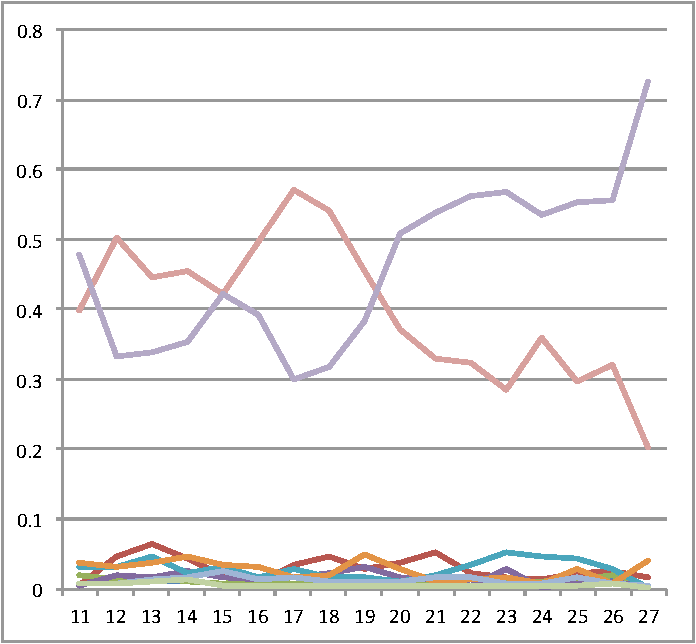
\includegraphics[width=0.48\linewidth]{figures/1LDANews-2.pdf}
%\label{fig:news_topics_lda}
%}
%\subfigure[\stlda]
%{
%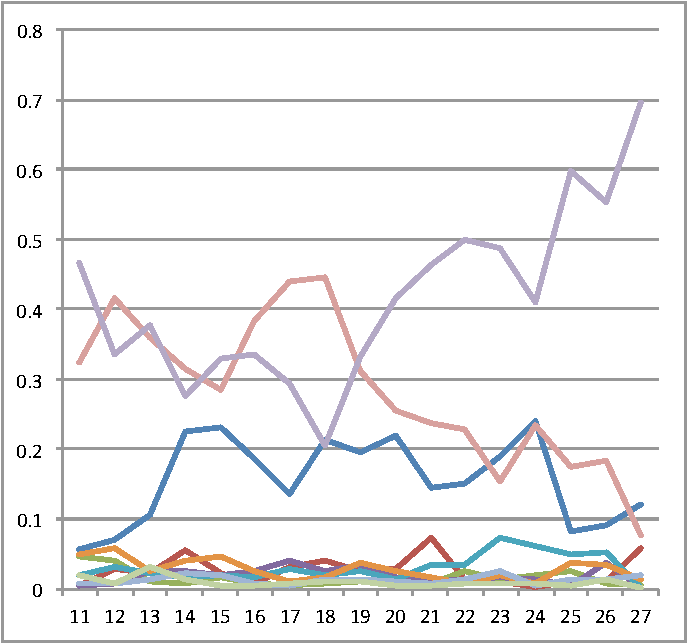
\includegraphics[width=0.48\linewidth]{figures/1STLDANews-2.pdf}
%\label{fig:news_topics_stlda}
%}
%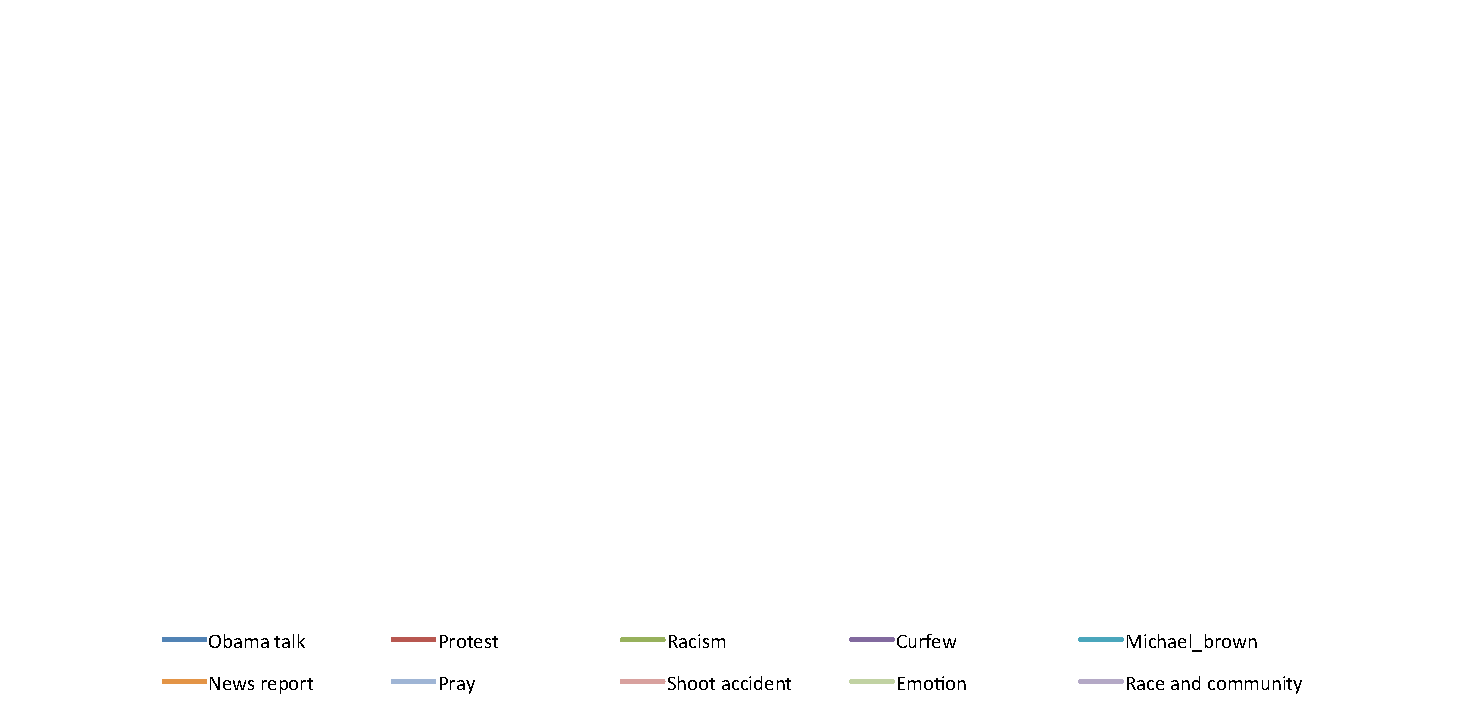
\includegraphics[width=\linewidth]{figures/Legend.pdf}
%\caption{News Topic Dynamics by LDA and \stlda}\label{fig:news_topics}
%\end{figure*}

%Topic distribution given by LDA is highly skewed to two main topics, thus the \shootincident and the \raceandcommunity, while other topics take only a small proportion and it is hard to identify the proportion change of these topics. Meanwhile \stlda gives results that are slightly better in representing different topics. Besides the significant change of \shootincident and \raceandcommunity, the \obamatalk is discovered as a main topic for media. It keeps a relatively stable proportion of 20\%, and peaks after some important events related with Obama. For example, on August 12, Obama addressed the shooting and urged the community in Ferguson to stay calm. On August 14, he gave a talk saying there is no excuse for protesters to turn to violence, which seems to lead to the peak on August 14 and 15. Also in news topic dynamics by \stlda, the \protest shows a peak on August 21, which is consistent with the date when the National Guard withdrew from the Ferguson.

%Both LDA and \stlda are unsupervised methods, so it is hard to verify which topic dynamic reflects the real situation. But the topics discovered by \stlda are more diverse, and are consistent with the important events in the timeline.

%There is more variance in topic dynamics of tweets by \stlda than LDA, which is shown in Figure~\ref{fig:tweets_topics}. The proportion of topics is close to each other in topic dynamics by LDA, so it is relatively hard to identify the main topics for each day. There is rising point of \michaelbrown after the shoot accident, and a peak on August 25 when the funeral for Michael Brown is held. However, consistent with the shortage discussed in analysis of tweet topics, LDA gives a probability distribution of topics, of which some are irrelevant. So when aggregating tweets in a day together, the proportion number for each topic is similar, which makes it hard to identify main topics on that day, and change of topics along the time. Comparatively, \stlda gives results with better representation of topic dynamics. There is variation of topics changing overtime. It is clearly that after the shoot accident, emotion of the public surges to a peak on August 11. After the protest event, another emotion topic appears on August 14. Meanwhile, the proportion of \pray topic keeps relatively stable from August 11 to August 24, and increases a lot on the day when Michael Brown's funeral is held. These tendencies in topic changes can be seen in topic dynamics of tweets by LDA, but these topics are entangled with other topics, making it hard to differentiate from other topics.

%\begin{figure*}[htpb]
%\centering
%\subfigure[LDA]
%{
%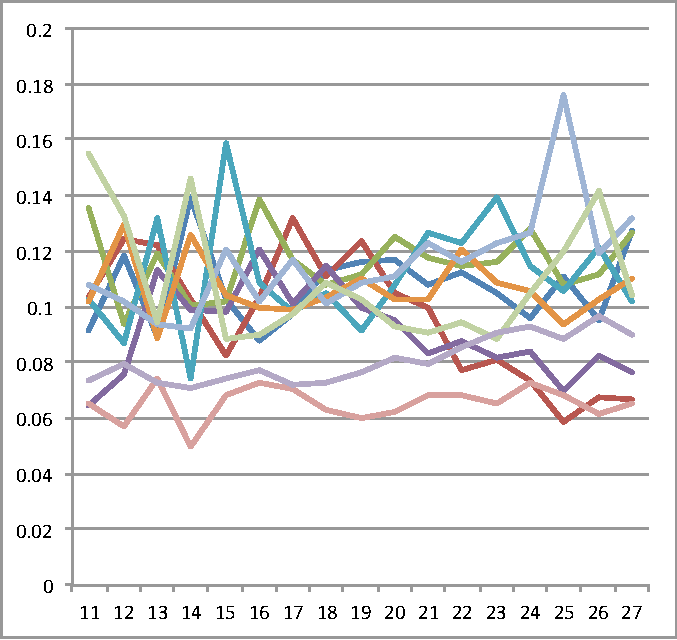
\includegraphics[width=0.48\linewidth]{figures/2LDATweets.pdf}
%\label{fig:tweets_topics_lda}
%}
%\subfigure[\stlda]
%{
%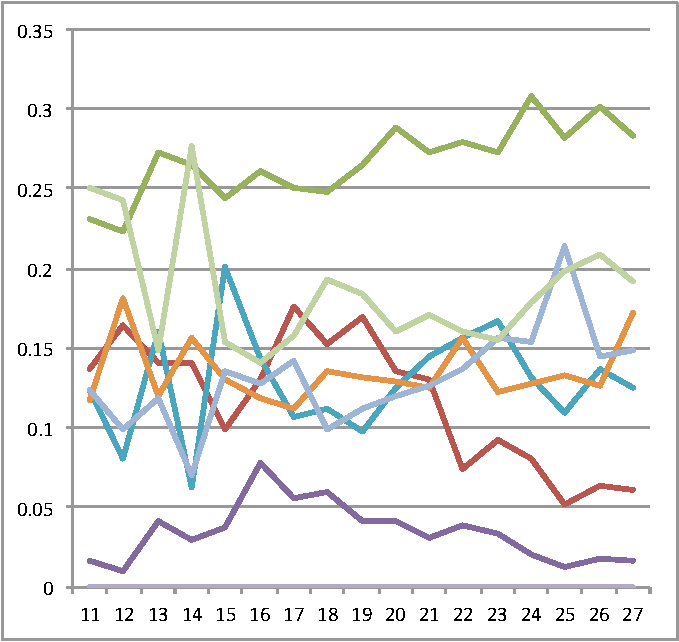
\includegraphics[width=0.48\linewidth]{figures/2STLDATweets.pdf}
%\label{fig:tweets_topics_stlda}
%}
%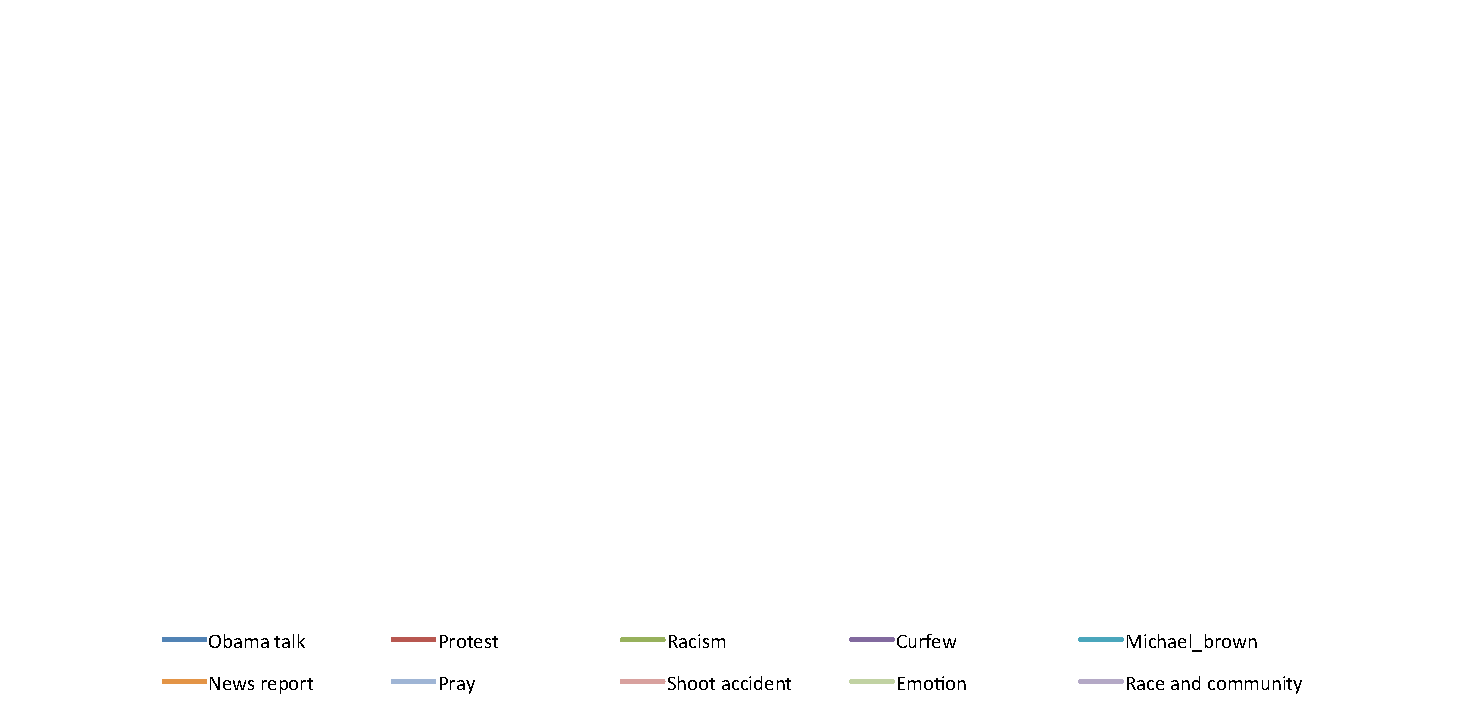
\includegraphics[width=\linewidth]{figures/Legend.pdf}
%\caption{Tweets Topic Dynamics by LDA and \stlda}\label{fig:tweets_topics}
%\end{figure*}

%In summary, by intrinsic and extrinsic evaluation, \stlda is more accurate in assigning one topic to each tweet and giving better results in topic dynamics. %In Section~\ref{subsec:topic_track}, we use the results of \stlda on tweets and news for topic tracking analysis.

